% Copied this sample latex file from https://www.usenix.org/conferences/author-resources/paper-templates
\documentclass[letterpaper,twocolumn,10pt]{article}
\usepackage{usenix,epsfig,endnotes}
\usepackage{array}
\newcolumntype{L}[1]{>{\raggedright\let\newline\\\arraybackslash\hspace{0pt}}m{#1}}
\newcolumntype{C}[1]{>{\centering\let\newline\\\arraybackslash\hspace{0pt}}m{#1}}
\newcolumntype{R}[1]{>{\raggedleft\let\newline\\\arraybackslash\hspace{0pt}}m{#1}}

\begin{document}

%don't want date printed
\date{}

%make title bold and 14 pt font (Latex default is non-bold, 16 pt)
\title{\Large \bf Kaggle Challenge: Predicting Rossmann Store Sales}

\author{
  {\rm Mingu Jo}\\
  University of California, Berkeley
  \and
      {\rm Wonjohn Choi}\\
      University of California, Berkeley
} % end author

\maketitle

% Use the following at camera-ready time to suppress page numbers.
% Comment it out when you first submit the paper for review.
\thispagestyle{empty}


\section{Abstract}
Our project attempted to apply linear regression and various machine learning techniques to a real-world problem of predicting drug store sales. Rossmann, Germany's second-largest drug store chain, has provided past sales information of 1115 Rossmann stores located across Germany. We preprocessed, feature-engineered the data, and examined 4 different statistical / machine learning analysis for forecasting sales of each store: multivariate linear regression, random forest, gradient boosting, and TODO. Then, we compared the methods' predictive power by computing Root Mean Square Percentage Error (RMSPE). We found that TODO:X performed the best with a RMSPE score of TODO:XXX.

\section{Introduction}
The objective of this project is to predict 6 weeks of daily sales for 1115 Rossmann stores located across Germany using the data which was provided by Rossmann through Kaggle. The motivation of this project is the following: by reliably predicting daily sales, store managers may decrease operational costs, and create effective staff schedules (ex. by assigning more staffs during busy days). Also, we would like to identify which type of techniques be effective in a real-world sales prediction task. Before building any regression or machine learning models for the prediction, we attempted to define which features are significant to determine daily sales of stores. By performing exploratory data analysis, we found how some features such as promotion and competitor distance affect the sales. % sounds little strange

To confirm our assumption and apply various techniques for the prediction, we first explored several similar efforts that made for sales prediction task in the past in order to set the basis of our study. 

- Linear Regression: The professor at Western Illionois University suggests multiple linear regression with feature selection and multicollinearity diagnostics to be a popuplar technique in sales forecasting. This model was applied for predicting the number of subscribers that a cable station can expect, which is closely related to our task. We decided to apply this technique along with partial t-test and stepwise regression to select significant features. 

- Random Forest: the random forest is a tree-based ensemble method where all trees depend on a collection of random variables. (Breiman). Breiman suggests that random forest algorithm is actually from a classification viewpoint but the approach is
applicable to regression as well. Therefore, we consider the algorithm is also applicable to our regression task. Nils Adriansson and Ingrid Mattsson in their thesis applies the algorithm into a GDP forecast task, showing its power in time-series forecasting (Adriansson). We assume this algorithm can outperform linear regression because Breiman states that the RF does not need to assume any distribution for variables. (Breiman)

- Gradient Boosting: We also found useful article by Jay Gu on gradient boosting regression. In his article, he asserted that, for predictive analytics, the gradient boosted trees model (GBM) is one of the most effective machine learning models. As he did, we have also witnessed a good number of winning solutions for various kaggle competitions that contain boosted tree models as a crucial component. We got the basic framework from the textbook (    ). Especially, we noticed that Extreme Gradient Boosting (xgboost) is similar to gradient boosting framework but more popular and efficient. We decided to fine-tune our dataset and apply the algorithm on it for better prediction.


\subsection{Description of Datasets}
Data sets are given by Rossmann through Kaggle. There are three files: test.csv, train.csv, and store.csv. train.csv contains 1017209 observed daily sales of different stores from 2013 to 2015. store.csv contains supplementary information for each store (41088 lines because there are 41088 stores). train.csv and store.csv both contain Store id that we can use to join the train and store data sets. Finally, test.csv has 41088 lines of daily sales of different stores but the value of Sales column is omitted. We are expected to predict the value of Sales column for the test set (test.csv) by using the training set (train.csv) and store data (store.csv).

The following table describes fields in test.csv and training.csv:

\begin{tabular}{| c | L{4cm} |}
  \hline
  Store & the unique id for each store (positive integer ranging from 1 to 1115) \\ \hline
  DayOfWeek & the day of week (positive integer ranging from 1 to 7 where 1, 2, ..., 7 correspond to Monday, Tuesday, ..., Sunday) \\ \hline
  Date & the date (string of format YYYY­MM­DD) \\ \hline
  Sales & the total amount of revenue for this given day (positive number between 0 and 41551). This value is what needs to be predicted, so only exists in training.csv. \\ \hline
  Customers & the number of customers on the given day. This also only exists in training.csv. \\ \hline
  Open & an indicator of whether the store was open on the given day (0 if closed, 1 if open) \\ \hline
  Promo & an indicator of whether the store was running a promotion on the given day (0 if not running, 1 if running) \\ \hline
  StateHoliday & an indicator of whether the given day was a state holiday (0 if not a state holiday, a if public holiday, b if eastern holiday, c if christmas) \\ \hline
  SchoolHoliday & an indicator of whether the store was affected by a nearby school holiday on the given day (0 if not affected, 1 if affected) \\ \hline
\end{tabular}

The following table describes fields in store.csv:

\begin{tabular}{| c | L{4cm} |}
  \hline
  Store & the unique id for each store (positive integer ranging from 1 to 1115) \\ \hline
  StoreType & the store's model (4 types: a, b, c, d) \\ \hline
  CompetitionDistance & the distance in meters to the nearest competing store (positive number franging from 20.0 to 75860.0, and NA's if no competitors) \\ \hline
  Assortment & the store's assortment level (a = basic, b = extra, c = extended) \\ \hline
  CompetitionOpenSinceMonth & the approximate month of the time when the nearest competing store opened (positive integer ranging from 1 to 12, and NA's if no competitors) \\ \hline
  CompetitionOpenSinceYear & the approximate year of the time when the nearest competing store opened (positive integer ranging from 1900 to 2015, and NA's if no competitors) \\ \hline
  Promo2 & an indicator of whether the store was participating in a promotion that runs over a period of time  (0 if not participating, 1 if participating) \\ \hline
  Promo2SinceWeek & the approximate week of year when the store started to participate in promo2 (positive integer ranging from 1 to 50, and NA's if no promo2) \\ \hline
  Promo2SinceYear & the approximate year of time when the store started to participate in promo2 (positive integer ranging from 2009 to 2015, and NA's if no promo2) \\ \hline
  PromoInterval & the months when the promo2 started (comma \\ \hline
\end{tabular}

\subsection{Preprocessing}

For preprocessing, we have done the followings:
\begin{itemize}
\item We merged train.csv and store.csv by ``Store'' because we can predict daily sales better with more data related to the sales. We also merged test.csv and store.csv by ``Store''.
\item We removed ``Customers'' field from the training data because it does not exist in the test data so we cannot use ``Customers'' to predict ``Sales''.
\item For ``CompetitionDistance'' with NA values, we replaced NA with 1000000. Since 1000000 is much more bigger than any other distances, replacing NA with the number simulated an effect of having no competitor. In the similar way, we filled missing values for ``CompetitionOpenSinceYear'' and ``CompetitionOpenSinceMonth''.
\item Similarly, for ``Promo2SinceYear'' with NA valus, we replaced NA with 1990 to simulate the effect of having no promo2.
\item We splitted ``Date'' field into three fields: ``year'', ``month'', and ``day''.
\item We computed average sales for each store to create a new field ``Average.Sales''.
\item We noticed the feature ``CompetitionDistance'' is highly skewed to right. For the sake of linear regression, we took log transformation on the feature ``CompetitionDistance'' to create a new field ``LogCompetitionDistance'' to make sure that the relationship between explanatory variables and dependent variable is approximately linear.
\end{itemize}

% TODO:add the CompetitionDistance graph here. 

\subsection{Exploratory Data Analysis}
To check any distinctive relationships between variables, we drew a pearson correlation coefficient plot using corrplot library. There are several interesting facts we captured. 
- ``DayOfWeek'' and ``Sales'' are negatively correlated. This implies that, as ``DayOfWeek'' approaches to Saturday and Sunday, sales would decrease because most drugstores would close on these days. 
- ``LogCompetitionDistance'' and ``Sales'' are negatively correlated. In other words, lower distance to the competitor implies slightly higher sales. We assume this could occur because stores with a close distance to the competitor are mostly located in crowded regions such as a downtown city with higher sales overall.

% TODO:add the correlation plot here. 



\section{Methods}
We started off by setting a benchmark to obtain a baseline for the prediction. Then, we took 3 different approaches to outperform the benchmark and former model.  

\subsection{5-fold Cross Validation}
To generalize our predictions to limit problems of overfitting on the training set, we decided to ramdomly partition the original training observations into 5 equal sized subsamples. The training set is comprised of 4 equal sized subsamples and the rest as the validation set. For the purpose of reproducibility and comparison of the predictive powers of different models, we set the seed (with a value of 42). Our general process would be as the following:
1. Repeat cross-validation process 5 times with each of the 5 subsamples used exactly once as the validation set.
2. Compute the average of 5 different validation error rate. 
3. Predict sales on the test set using the model. 
4. Submit on Kaggle website to get the test error rate.
5. Compare the average validation error rate and the test error rate among differnent models.


\subsection{Error Metric}
As the metrics that Kaggle uses to compute test error is the Root Mean Squared Percentage Error (RMSPE), we used the same metrics to compute our validation error. It's the following:

$RMSPE = \sqrt{\frac{1}{n} \sum {(\frac{y_i - \hat y_i}{y_i})}^2}$

where ${y_i}$ is a store's sales on a single day, ${yhat_i}$ is the daily sales prediction for the store on the day, and ${n}$ is the number of (store, date) pairs in the data set. 

\subsection{Benchmark}
Our benchmark is simply the average sales of each store. Precisely, we predict daily sales of a store for a day by the average daily sales the store had in the training data set. This method does not account for many factors (whether the day was holiday, whether the store was running a promotion on the day, etc), so we expect its error rate to have a higher error rate than any other methods we applied.

\subsection{Linear Regression}
Linear regression is an approach for modeling the relationship between dependent variable Y (in our case, ``Sales'') and explanatory variables X. To apply linear regression on the data, we decided to use R's $lm$ function. $lm$ is an implemention of multivariate linear regression. If we supply $Y \sim X$ as the input, $lm$ builds and returns a model that can be used to predict $Y$ using $X$. Under the hood, it basically solves the normal equation $\beta = (X^T X)^{-1} X^T Y$.

We first built linear model with all available features (DayOfWeek, Open, Promo, StateHoliday, SchoolHoliday, StoreType, Assortment, CompetitionOpenSinceMonth, CompetitionOpenSinceYear, Promo2, Promo2SinceYear, Average.Sales, LogCompetitionDistance, CompetitionDistance, day, month, year) using the training set. Then, we applied the linear model on validation set.

\subsubsection{Feature Selection}
Then, we did feature selection to reduce complexity of linear model. Before working on feature select, we took a look at the resulting lm with R function $summary(lm)$ to get some general idea of how important each variable is. All features except CompetitionDistance, CompetitionOpenSinceMonth, CompetitionOpenSinceYear, Promo2, Promo2SinceYear were significant with p-value less than 0.05.

\subsubsection{Feature Selection-Backward Elimination}
For feature selection, we first applied backward elimination by repeatedly removing features with the highest p-value until no feature has p-value higher than 0.05. As the result, we obtained DayOfWeek, Open, Promo, StateHoliday, SchoolHoliday, StoreType, Assortment, Average.Sales, LogCompetitionDistance, day, month, year. Then, we built linear model with the selected variables using the training set and applied linear regression with the model on the validation set.

\subsubsection{Feature Selection-Akaike Information Criterion}
Another approach we had for feature selection was using Akaike information criterion (AIC). AIC provides a meature of relative quality of models with the equation $AIC = 2k - 2 ln(L)$ where $k$ is the number of estimated paramters in the model and $L$ is the value of likelihood function. We performed AIC by using R function $stepAIC$.

\subsubsection{Feature Engineering-Lasso}

\subsubsection{Feature Engineering-Ridge}


\subsection{Random Forest}
Random Forest is an ensemble learning method that constructs decisions tree using training set. By aggregating many decision trees, Random Forest can make predictions while avoiding overfitting because it uses an ensemble of regression trees over different samples of the data. Here is our Random Forest Regression steps: \\
\begin{enumerate}
\item Construct random forest trees (number of trees is defined by hyper parameter)
\item Classify the incoming data into the decision tree node
\item Calculate the mean value for each node for prediction
\end{enumerate}

In particular, we used H2O’s RandomForest package to carry out the training and prediction. Then, we optimized parameters to improve on our prediction model. H2O is the open source math engine for huge dataset (TODO). Since H2O package enables us to compute Random Forest Regression algorithm in parallel distribution, we decided to use the package for faster computation compared to R's Random Forest package.

To find the best hyperparamters, we tried different values of hyperparamter and tested the results on validation set using for loops.

\subsection{Gradient Boosting}
The similarity between Random Forest and Gradient Boosting is that both generate decision trees. However, Random forest uses bootstrapping method for training while Gradient Boosting builds decision tree over the residuals. In other words, Gradient Boosting Tree generates the decision tree as it optimizes on a proper loss function (   ). This refers that we can establish our own loss function for optimization, while we couldn't do in Random Forest. We set our loss function to be our error metric, RMPSE. Our decision trees here are regression trees. Each regression tree divides the data point at each non-leaf node according to a constraint on a feature. The leaf node value of a data point decides its score, and a data point is predicted by averaging the scores of the leaf node it belongs to.

In particular, we used R's xgboost package. XGBoost also known as Extreme Gradient Boosting is a powerful supervised learning algorithm (). This package enables an automatic parallel computation on a single machine. For our regression task, we put ``reg:linear'' as a parameter. Our training objective here is :

at most d times, since we might have to try up to d values for Xj before finding a solution

\section{Supplementary Methods}

\section{Results}
\subsection{Benchmark}
Our benchmark is the average sales of each store. The error rate for benchmark was 0.106209 on validation set and 0.25789 on the test set (when submitted to Kaggle website). This is our baseline model. Our goal is to improve our prediction by outperforming the benchmark by large degree at the end. 

\subsection{Linear Model}
The error rates of our different linear models are following:

\begin{center}
    \begin{tabular}{| l | l | l |}
      \hline
       & Validation Error & Test Error \\ \hline
      Linear Regression \\
      (Full Model) & 0.09101 & 0.21036 \\ \hline
      Linear Regression \\
      (Backward Elimination) & 0.09108 & 0.20988 \\ \hline
      Linear Regression \\
      (AIC) & 0.091006 & 0.21039 \\ \hline
      \hline    
    \end{tabular}
\end{center}

We also wanted to check which features were actually removed by the feature elimination methods. 

TODO blah blahblahblah features blachblashblash 


\subsection{Random Forest}
The major parater we tune for Random Forest is the depth and number of trees. We used 5 fold cross validation to compute average RMSPE while varying the depth and number of trees. The plot for varying depth is shown below:

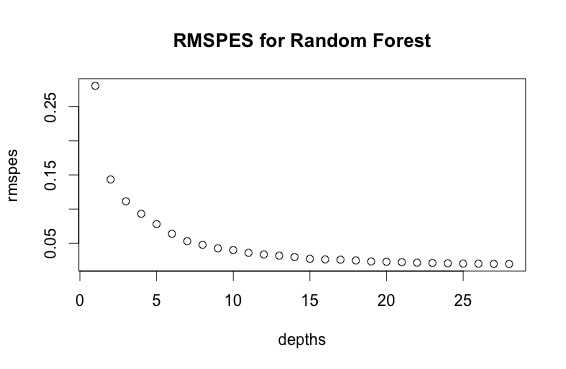
\includegraphics[scale=0.35]{img/RandomForestPerDepth.png}

As the plot illustrates, we see that RMSPE does not change much after depth reaches 20. Also, we confirm that the test error rate 

The plot for varying ntrees is shown below:

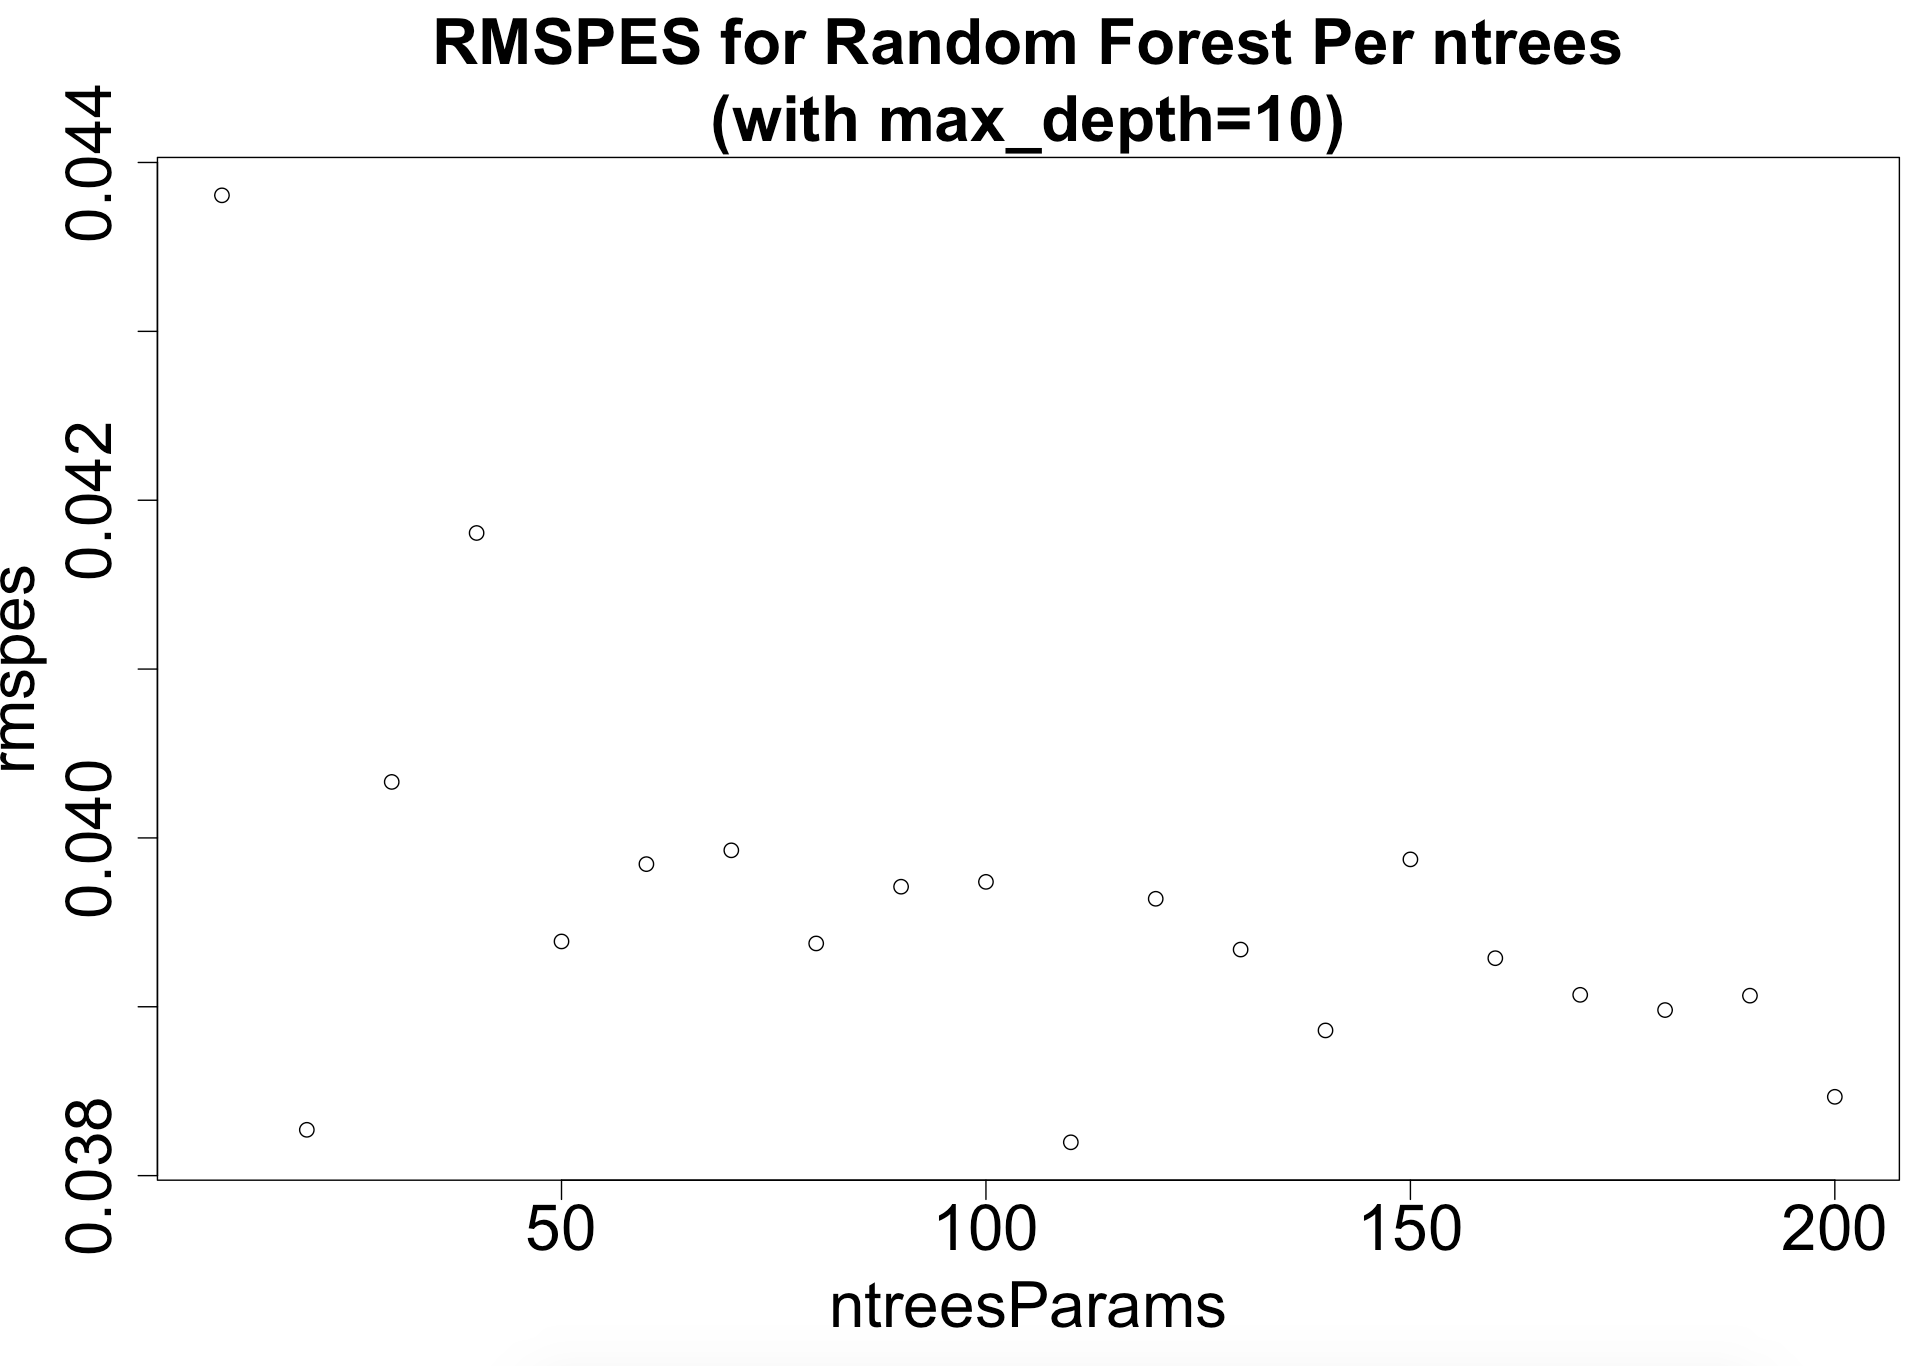
\includegraphics[scale=0.35]{img/RandomForestPerNtrees.png}

We see that unlike depth, ntrees does not have much impact on RMSPE (TODO).

As the plot illustrates, we could see that RMSPE does not change much after the number of tree reaches TODO. Also, we could confirm that the test error rate does not increase even if the number of trees reaches as big as TODO. This is because Random Forest tree utilizes random amount of the data for training. In the algorithm, the training set for a tree is drawn by sampling with replacement.

Hence, we chose 30 as depth, 100 as ntrees to run random forest. The error rate for random forest (depth=30, ntrees=100) was 0.020639 for validation set and 0.14411 on test set.

\subsection{Gradient Boosting}
Before comparing the results of gradient boosting with other algorithms we performed, let's explore on the results of gradient boosting itself only. Although we already feature engineered our data set, we decided to also see how our test error rate changes when we exclude stores with 0 sales. As we did in previous methodologies, we tried a range of certain parameters to maximize its prediction accuracy. Since the major issue of all machine learning tasks is to prevent overfitting on training data, we also used 5-fold cross validation to generalize. We computed the average error rates of 5-fold as a parameter changes, and graphed them to choose the best parameter. There are actually more parameters to tune in Gradient Boosting. There are three major parameters subject to be tuned: the step size of each boosting step (learning rate), maximum depth, and the max number of iterations. For our task, we decided to use the default number of trees and max number of iterations, but tune the step size. We might check how the different number of iterations affect the performance, but we checked it did not affect much but exponentially increase the runtime. We decided to set it as 300, and try different step sizes. 

The effects of tuning the step size are visualized in the following graph:


As the error rate shows, Gradient Boosting model gives us the most predictive power by far. We were able to achieve test error rate (RMPSE) of 0.13234.


\section{Supplementary Methods}

\section{Discussion}
To visualize the overall performance of our different models, we organized the resulting error rates into a simple table. 

% TODO: make an overall error rate table
\begin{center}
    \begin{tabular}{| l | l | l |}
      \hline
       & Validation Error & Test Error \\ \hline
      Benchmark & 0.106209 & 0.25789  \\ \hline
      Linear Regression \\
      (Full Model) & 0.09101 & 0.21036 \\ \hline
      Linear Regression \\
      (Backward Elimination) & 0.09108 & 0.20988 \\ \hline
      Linear Regression \\
      (AIC) & 0.091006 & 0.21039 \\ \hline
      Random Forest & 0.020639 & 0.14411.  \\ \hline
      Gradient Boosting & 0.01734 & 0.13234  \\ \hline
      \hline    
    \end{tabular}
\end{center}

Although we readily outperformed our benchmark, as we expected, linear regression model did not perfrom very well because of the non-linearity of the data. However, we checked the sharp increase from linear regression to Random Forest model. we confirmed that tree based models can approximate functions with any ``non-linear shape'', whereas linear models can produce functions with a ``linear shape'' with respect to a chosen set of features. 

There were TODO features removed by feature selection method. We think TODO 

As a result, we were able to achieve TODO RMPSE using gradient boosting to predict Rossmann drugstore sales without using customer number information. Although boosting performed very well for this dataset, we witnessed it's harder to tune parameters and took longer time to train the data compared to Random Forest. While the number of tree is only usually tuned to train Random Forest, Gradient Boosting model requires several parameters to be tuned. In addition, tuning such parameters and comparing corresponding performances requires much more time than computing Random Forest algorithm. Also, Random Forest does not easily overfit. Often, many statisticans say Random Forests does not overfit. The testing performance of Random Forests does not decrease (due to overfitting) as the number of trees increases (Breiman). However, Boosting algorithm is more robust to overfitting because it relies on every single data point and tries to find optimal linear combination of regression trees given the train dataset. Thus, it requires proper tuning to avoid it. As shown in the table, it took more than 5 hours to train Gradient Boosting model, and compute different error rates according to different parameters over 5-fold cross validation. We could have potentially increased the size of the number of tree and get better precision, at the risk of overfitting and longer training time which is a tradeoff between time and accuracy.

In conclusion, we can check that our well-tuned gradient boosting model outperformed Random Forest. 

\section{References Cited}

Dehkordi-Vakil, Farideh. "Multiple Regression Analysis." DS-533. Illionis, Macomb. Lecture.

Breiman, L., (2001a). ”Random Forests”, Machine Learning 45 (1) pp. 5-32.
R.D. https://www.diva-portal.org/smash/get/diva2:785776/FULLTEXT01.pdf


https://documents.software.dell.com/statistics/textbook/boosting-trees-regression-classification

h2o package description


\section{Author Contributions}

\end{document}
}



